\chapter{Results}

\begin{comment}
In this chapter I will present the results of my analysis.\\
Software:\\
Software engineering:\\
-what issues with the structure of different openMNGlab version did I encounter\\
-What are the needs of different users of the framework in the end?\\

Spike Analysis:\\
-Describe quantifiers and discuss the results of analysing the experimental recordings\\
-image of table containing everything the jupyter notebook has computed\\
-table with info on electrical frequency levels in each recording\\
-diagram showing a quantifier (peak firing frequency) and electrical frequency for each spike train of single recording\\
-compare diagrams of different recordings\\
-compare different quantifiers in one diagram with each other for the same file\\
-compare ISI to log(ISI) for every train in one file\\
\end{comment}


\section{Software}
\subsection{Finished analysis pipeline}
The software development process described in the previous chapter resulted in a jupyter notebook, which represents the current analysis pipeline used for the analysis in this thesis. A schematic version of this pipeline can be seen in figure TODO. For a more detailed view on the different functions, have a look at a more detailed diagram or the code in the appendix. 
\subsubsection{Importing data}
The first part of the notebook is the import of the data, which consists of two separate importing steps. 
First we use the Neo importer from the current version of our framework to extract the information about the underlying electrical stimulation. After that we use the importer from the old version of openMNGlab to get the spike timings as well as the information about the mechanical stimuli.
After the two importing steps we end up with two separate data structures, that we discussed in the previous chapter, each containing part of the experimental data. From the first importing step, we get the event information about the electrical stimulation in the Neo format. The mechanical stimuli with its physical properties such as amplitude and duration, as well as the spike timings, we receive with the second importing step. This information is contained in the custom data structure. The spike timing would also have been available in the newer Neo format, however, the analysis code was started with the custom data structure in mind, so I did not change that part of the code for the purposes of this thesis. For the future it would be a good idea to switch fully to the Neo structure, so that there is a unified structure for everything.\\
% spike2 csv export to import for additional custom structure
\subsubsection{Preprocressing}
The next part of the notebook contains internal processing steps to sort the spike trains and prepare the data for easy representation and quantification.\\
Making use of the early versions of OpenMNGlab and the first analysis notebooks from Radomir the event plot for the current file gets computed and visualized. The next step is calculating the inter spike distances, meaning the time between two spikes, and creating inter spike distance graphs for each spike train in the recording.\\
\subsubsection{Computing quantifiers}
Now follows the main part of quantifier computation. This is where the computations of my chosen quantifiers happens. After all the quantifiers are computed the resulting lists of quantifiers for each spike train get put into a data structure and saved for later reimporting and reuse for further analysis.\\
\subsubsection{Visualizations}
Now that the quantifiers are calculated it is time to visualize the results. For this, I create different diagrams showing quantifiers over the whole recording and comparisons of different quantifiers. These figures will be explained in the analysis part of this chapter.\\
%See the appendix for a detailed view of the whole notebook as well as the code.



\section{Spike Analysis}
We have analyzed 22 recording files featuring  mechanical and electrical stimulation. An overview for the data can be found in  Table~\ref{table:recording_overview}. Here we see the number of spike trains in each file and the average spikes per train as well as the average spike train duration. More information about the specific recordings is following in the next section.

%\begin{comment}
\begin{table}[!ht]
\centering
\begin{tabular}{ |c|c|c|c| }
	\hline
	File number & Number of trains  & Avg. spikes per train & Avg. train duration\\
	\hline
	1 & 17 & 12.53 & 0.38 \\
	2 & 34 & 16.62 & 0.39 \\
	3 & 37 & 20.03 & 0.40 \\
	4 & 12 & 4.67 & 0.28 \\
	5 & 11 & 9.18 & 0.25 \\
	6 & 22 & 8.55 & 0.12 \\
	7 & 17 & 10.82 & 0.38 \\
	8 & 16 & 7.38 & 0.40 \\
	9 & 28 & 12.93 & 0.37 \\
	10 & 35 & 8.83 & 0.35 \\
	11 & 37 & 15 & 0.41 \\
	12 & 31 & 13.45 & 0.38 \\
	13 & 18 & 10.28 & 0.24 \\
	14 & 22 & 35.64 & 0.44 \\
	15 & 32 & 13.91 & 0.13 \\
	16 & 32 & 25.53 & 0.39 \\
	17 & 33 & 30.45 & 0.23 \\
	18 & 33 & 29.30 & 0.31 \\
	19 & 31 & 11.74 & 0.38 \\
	20 & 48 & 10.85 & 0.40 \\
	21 & 51 & 22.8 & 0.24 \\
	22 & 50 & 12.16 & 0.36\\
	\hline
\end{tabular}
\caption{This table shows a little overview over the available recording files for this thesis.}
\label{table:recording_overview}
\end{table}
%\end{comment}

\subsection{Experimental Protocol}
This subsection will explain how the recording files are structured to get a better general understanding of the experiments and analysis.

As mentioned in previous chapters, the files I am working with feature electrical and mechanical stimulation. Mechanical pressure is applied to the nerve fiber with a mechanostimulator described in~\cite{roberto} in a sinosoidal shape as can be seen in Figure~\ref{fig:spike_train}. The attributes of this type of stimulation, like amplitude or duration, is constant over the course of single recordings, but may change  for different recordings. In addition to the mechanical stimulation there is also electrical stimulation, which is applied as electrical impulses with a certain frequency. The base frequency of the electrical stimulation is the same for each of the recordings and lies at $0.1$ Hertz. This base frequency is applied during the whole recording with a few exceptions. Each recording features segments where there is electrical stimulation with increased frequency, during which a varying number of spike trains take place (usually $5-6$). After each of those segments with increased electrical frequency there is a smaller period of stimulation where the frequency is at $0.5$ Hertz before it goes back to the base frequency. One spike train get triggered during each of these small periods. In the recordings that where analyzed in this thesis there are 3 different levels of increased electrical stimulation frequency, which lie at $2.0, 4.0$ and $5.0$ Hertz.\\
Each file features at least one burst of increased frequency at one of the mentioned levels. The files in Table~\ref{table:recording_overview} are ordered according to the frequencies of electrical stimulation that occurred in the recordings. Files $1-3, 4-12, 13-14$ contain only frequencies of $2.0, 4.0, 5.0$ Hertz respectively. Files $15-20$ contain both $2.0$ and $4.0$ Hertz frequencies and files $21-22$ contain all three types of increased frequencies.\\

\subsection{Sample Analysis}
To show the results of the analysis in more detail I will use recording 21 as an example and demonstrate the outcomes. This will give a good look at the quantifiers that I chose to utilize as well as present possible visualizations using those quantifiers.

\subsubsection{Table of values}
When applying the analysis notebook to a recording, the first basic output we get is a big table containing the finished quantifiers as well as the original timestamp values for the spikes. A sample table can be seen in Table~\ref{fig:table_sc}, which shows a screenshot of the output table for recording 21.
First of all the table contains the mechanical stimulus information for each train. This includes the amplitude, duration and timestamp of the corresponding stimulus. In the figure this information is contained in the upper third of the table.
In addition the table features the single value quantifiers for the spike trains that I described in the previous chapter. These include among others the peak firing frequency, spike count and mean firing frequency and can be found in the middle third of the figure.
Lastly the table also features some of the raw data such as the spike timings as well as some intermediate results such as the inter pike intervals, which can be used to compute some of the single value quantifiers. These are depicted in the lower third of the figure in an abbreviated version for the sake of visibility.\\
\begin{figure}
	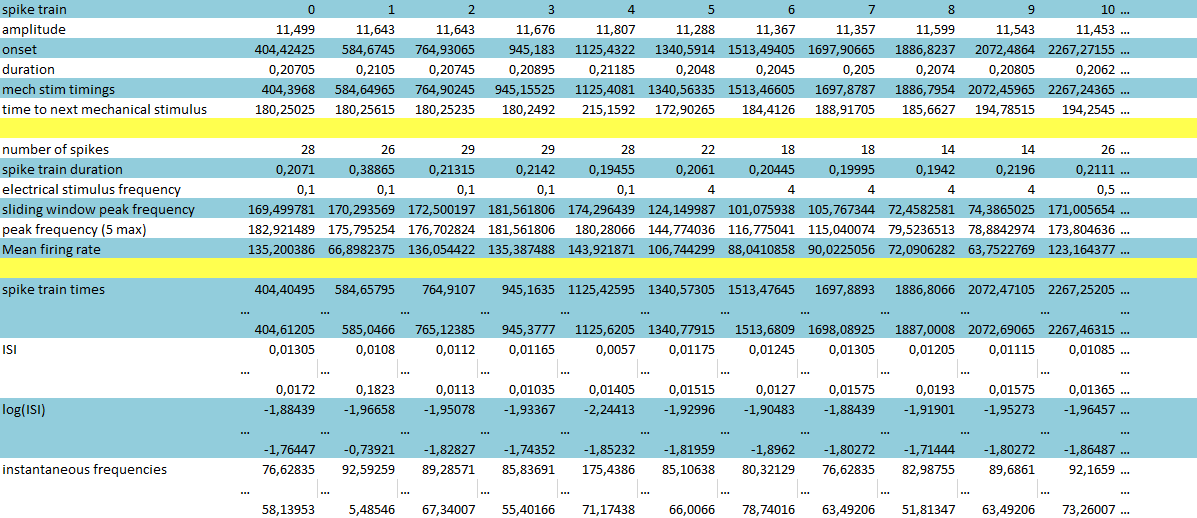
\includegraphics[width = \textwidth]{src/pic/sc_table}
	\caption{Sample picture of table after successful analysis }
	\label{fig:table_sc}
\end{figure}

\subsubsection{Event plot}
A figure that we have seen previously in this thesis is the event plot \ref{fig:eventplot}. It shows an overview of spiking activity after mechanical stimuli over the course of a whole recording. It is not meant to be an in depth analysis tool, but rather a quick visual representation of a recording. This can give us an idea if it makes sense to further analyze a particular recording, by looking at the length of the spike trains.

\subsubsection{Comparative diagrams for quantifiers}
Having computed the quantifiers is all well and good, but now we want to visually compare them in order to see if there is correlation between them in any way.
\begin{figure}
	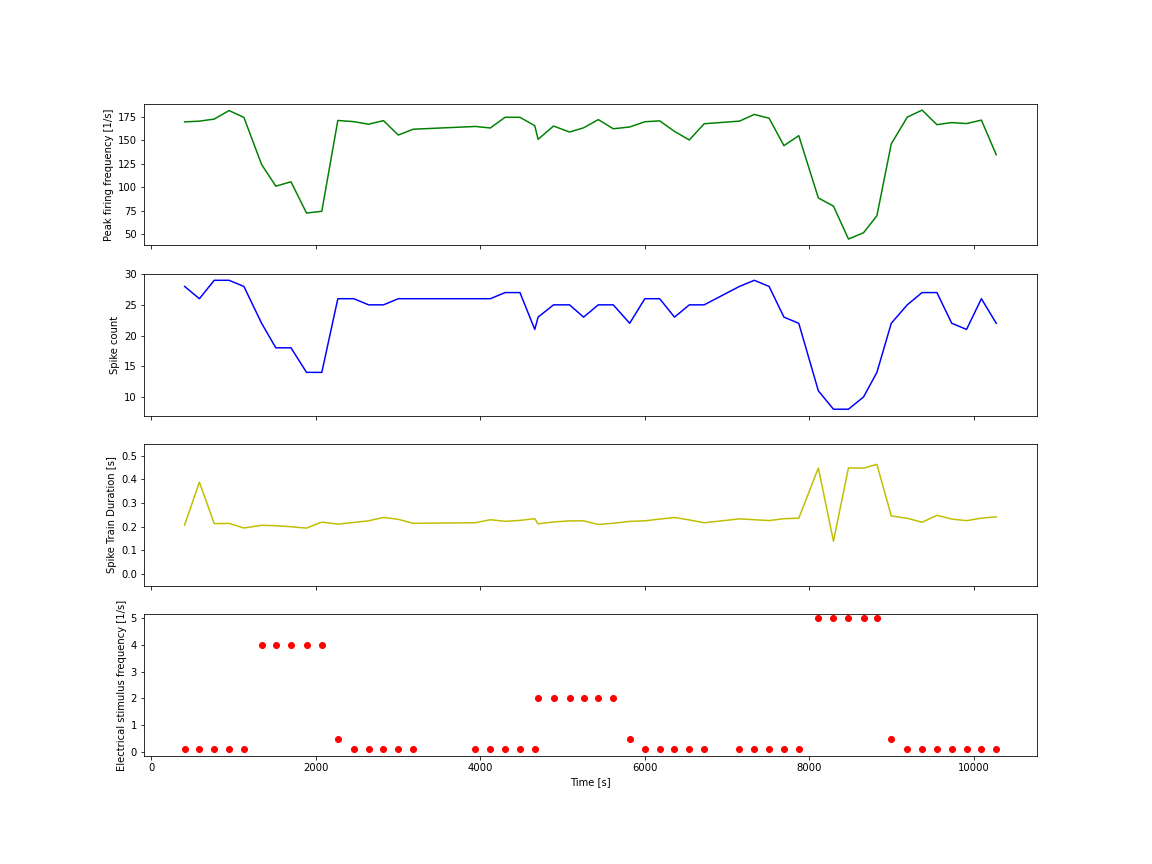
\includegraphics[width = \textwidth]{src/pic/11_12_13_sp}
	\caption{Diagram showing a separated comparison of peak firing frequency and spike count for recording 21}
	\label{fig:quantcomp_sp}
\end{figure}
\begin{figure}
	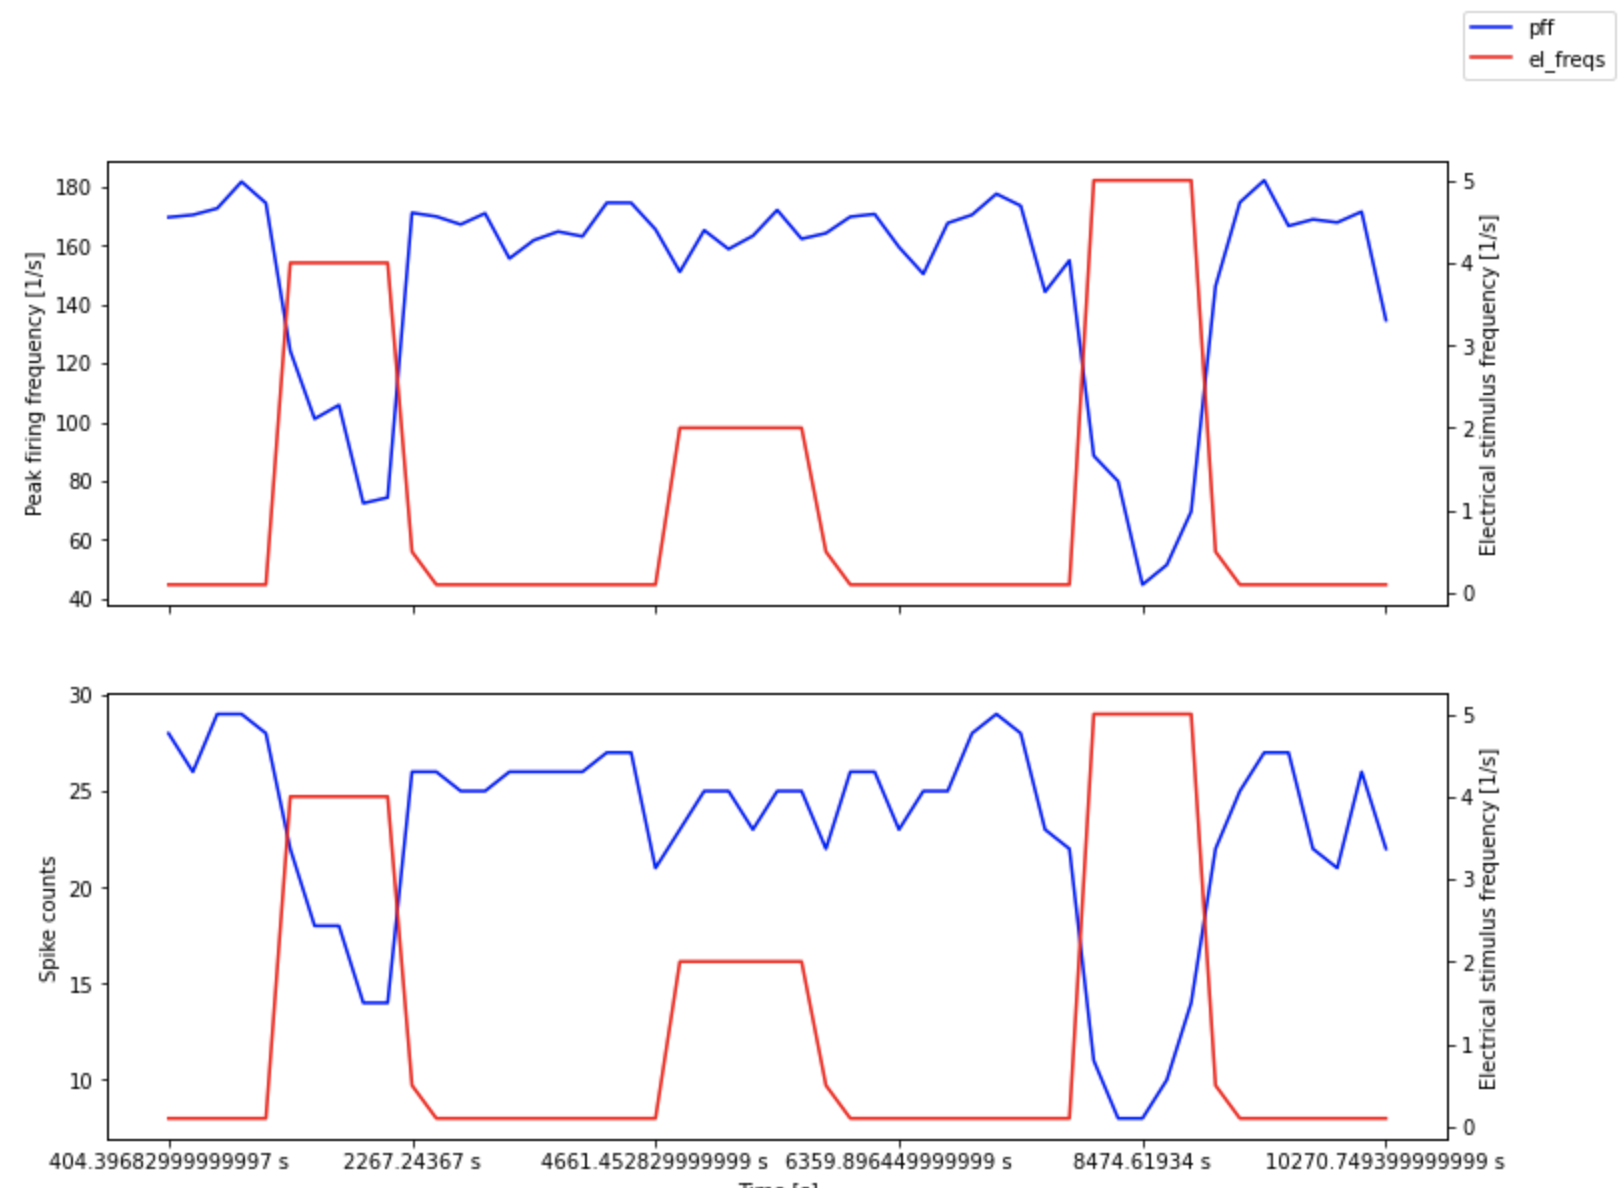
\includegraphics[width = \textwidth]{src/pic/11_12_13_cm}
	\caption{Diagram showing a comparison of peak firing frequency and number of spikes for recording 21}
	\label{fig:quantcomp_cm}
\end{figure}

A good visualization of this can be seen in figure~\ref{fig:quantcomp_sp}. This figure compares the spike count with the Peak firing frequency in recording 21. The time is plotted on the x axis ranging from the start of the recording to the end. This recording lasted over 10000 seconds. For each spike train we plotted the Peak firing frequency, the spike count as well as the Spike train duration in separate rows of the figure. In addition we added the electrical stimulation frequency, to see what effect the changes in frequency have on different quantifiers. Figure~\ref{fig:quantcomp_cm} shows the same data in a slightly different format. Here the electrical stimulation frequency is included in the rows where we plot the quantifiers to better see the immediate effect.\\
The first thing that we can observe is that the Peak firing frequency and spike count behave very similarly and have almost the exact same graph. Secondly, the application of different electrical stimuli does seem to have an effect on the spike trains. We can see that in the areas with 4 and 5 Hertz stimulation the peak firing frequency as well as the spike count take a significant dip. However, the same cannot be said for the interval with 2 Hertz stimulation. The quantifiers stay largely the same, which leads us to the assumption that there is some sort of threshold which needs to be passed in order to influence the spike trains. In our recordings this threshold seems to lie somewhere between the 2 and 4 Hertz electrical stimulation marks.
While the peak firing frequency and spike count show significant variation, the pike train duration stays pretty constant for the 4 Hertz stimulation but does also increase during 5 Hertz stimulation. This may point to different thresholds for different aspects of a spike train.

\subsubsection{Instantaneous frequencies}
\begin{figure}
	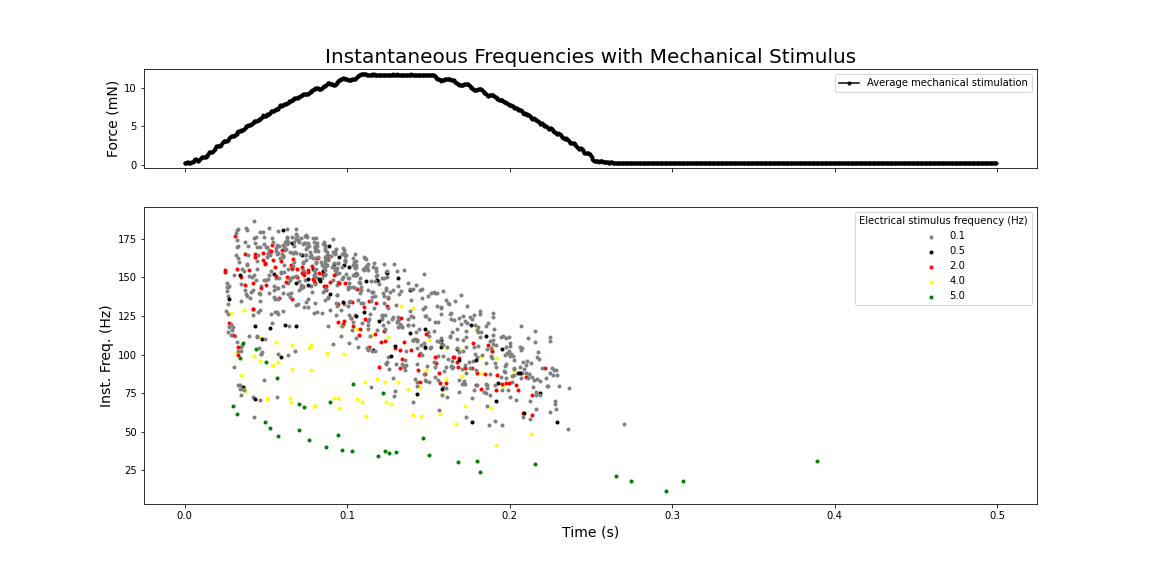
\includegraphics[width = \textwidth]{src/pic/11_12_13U1b_inst_freqs}
	\caption{Figure showing the instantaneous frequencies in each spike train for one recording.}
	\label{fig:inst_freqs}
\end{figure}
Another quantifier that we can take a look at is the instantaneous frequencies of the spikes in the spike trains and observe how these change with different levels of electrical stimulation. To visualize this we recreated a figure from the original paper from Roberto de Col in Figure \ref{fig:inst_freqs}. The data for this figure is taken from recording 21. The x axis depicts the time since the last stimulus in seconds. The top part of the figure shows the force of mechanical stimulation that evoke the spike trains. This curve represents the average mechanical stimulus in this recording. A sliding window of three was used for the calculation of the instantaneous frequencies to smooth out some of the outliers. The lower part of the figure is a scatterplot of these instantaneous frequencies for every spike train in the recording. They were color-coded according to the underlying electrical stimulation frequency. The pike trains with the base level frequency of 0.1 Hertz are colored in gray, while the trains with higher stimulation are colored in red, orange and yellow for an electrical frequency of 2, 4 and 5 Hertz respectively. Finally the trains with a stimulation of 0.5 Hertz stimulation frequency are colored in blue. From the scattering of the dots we can observe that the spike trains occurring during an electrical stimulation of 4 and 5 Hertz show lower instantaneous frequencies than the base level spike trains. The red dots lie mostly in the main cluster of dots belonging to the base level spike trains, which would fit with the previous figures and the assumption of some sort of threshold for spike train alterations.



%-diagrams of Interspike Intervals(isi) and logarithm of isi\\
%-should show that by taking the logarithm, the isi becomes more linear\\




\cleardoublepage
